\section{Evaluation}
\label{sec:evaluation}

\subsection{Hypotheses}
The primary hypothesis is that the motion of speckle patterns can be effectively visualized using a photodiode array. 
Additionally, it is hypothesized that the use of multiple lasers will influence the signal-to-noise ratio (SNR) of the measurements.

\subsection{Apparatus}

The custom-designed PCB transmitted its analog signals to an 8-channel Digilent ADC MCC 128 DAQ Hat, which was powered by a 5V low-noise bench power supply. 
A piezo disc, positioned at a distance of approximately 30~cm, was excited using a signal generator set to produce a sine wave at 133~Hz with a peak-to-peak amplitude of 3~V. 
All lasers utilized in the setup operated at a wavelength of 850~nm.

For visual alignment of the lasers, one camera was employed, while another camera was used to monitor the presence of speckles. 
Both the cameras and the photodiode array were equipped with 8~$\times$~8~$\times$~1~mm bandpass filters at 850~nm with a 40~nm FWHM and a 90\% transmission rate (manufacturer: Haian Subei Optical Glass Factory).
Data acquisition was handled by a Raspberry Pi, which recorded the ADC data. 
Data processing was performed in real time during qualitative experiments or recorded for later post-processing.

\begin{figure}[t]
\centering
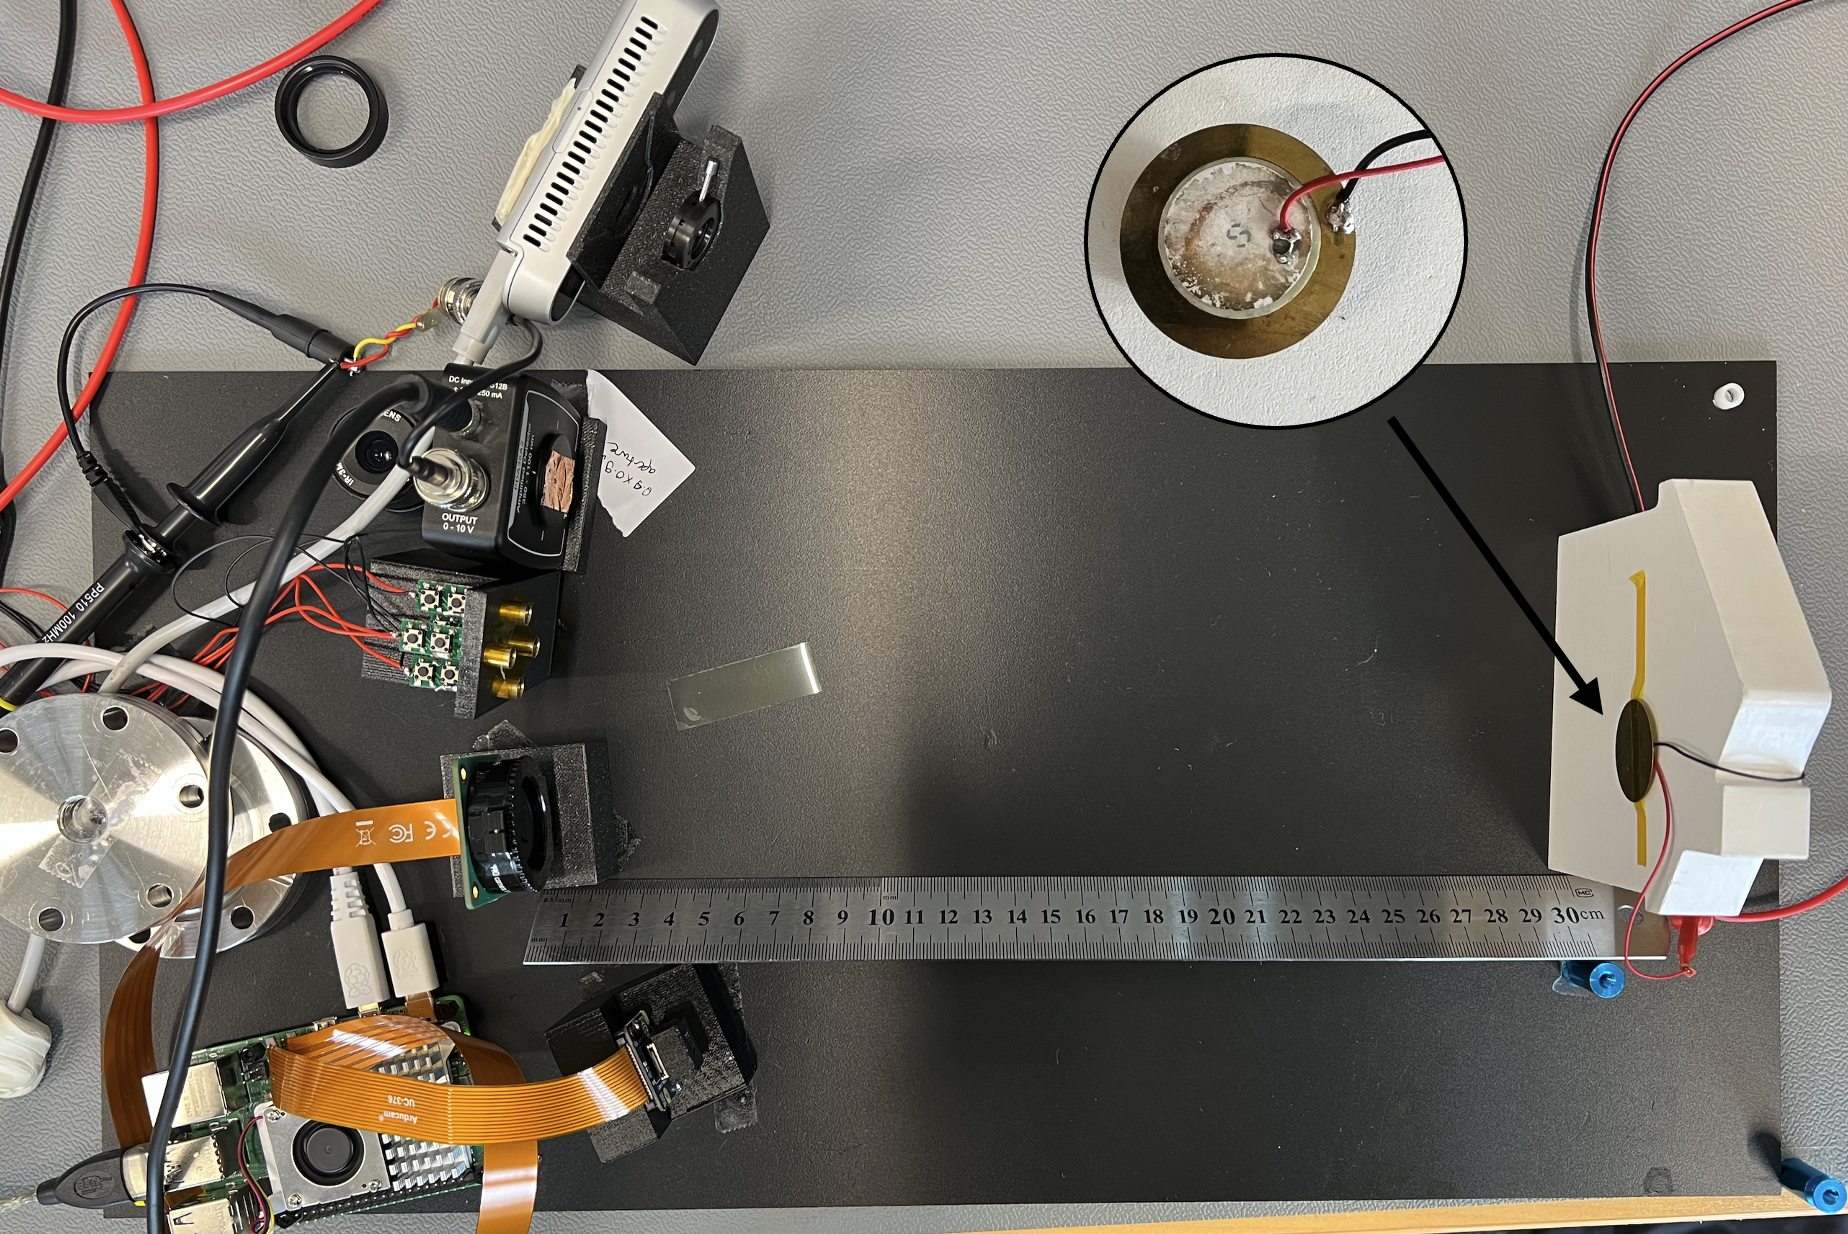
\includegraphics[width=\widthnarrow]{figures/eval/typical_setup.png}
\caption{Photo of the experimental configuration with the piezo disc.}
\label{fig:setup}
\end{figure}

\subsection{Procedure}

The initial steps of the evaluation involved SPICE simulations to analyze the Bode plot and transient response of the amplifier, as illustrated in Figures~\ref{fig:bodeplot} and \ref{fig:transient}. 
These simulations provided the theoretical SNR and total noise values (Figures~\ref{fig:totalnoise} and \ref{fig:snr}), demonstrating that the amplifier displayed stable behavior with high gain. 
Based on these results, the PCB was constructed.

Following the PCB assembly, it was meticulously cleaned using isopropyl alcohol (IPA) and compressed air, particularly under the pads of the amplifier section. 
Removing all flux residue from the PCB was deemed critical to ensure accurate operation. All measurements were conducted in a light-controlled environment to minimize interference from external light sources.

To assess the influence of multiple laser sources, a controlled surface vibration of the piezo disc at 133~Hz was measured while lasers in the square array were activated incrementally (Figure~\ref{fig:lasers}). 
For each configuration, the power spectral density of the inter-channel variance signal was calculated, and the SNR was analyzed. The spectral analysis, shown in Figure~\ref{fig:laser_snr}, 
established a positive correlation ($R^2 = 0.60$) between the number of active lasers and the detection SNR. 
A control measurement with all lasers switched off confirmed that the recorded signals originated from laser speckle patterns.

Additionally, time-domain signals captured by multiple photodiodes were compared to verify that each photodiode detected phase-shifted signals, which indicated the presence of a moving speckle pattern. 
An infrared (IR) LED was integrated into the setup to validate that the observed vibrations were dependent on coherent light.

\begin{figure}[t]
\centering
\includegraphics[width=\widthnarrow]{figures/eval/transient}
\caption{Transient response captured during SPICE simulation, highlighting amplifier dynamics and stability.}
\label{fig:transient}
\end{figure}

\begin{figure}[t]
\centering
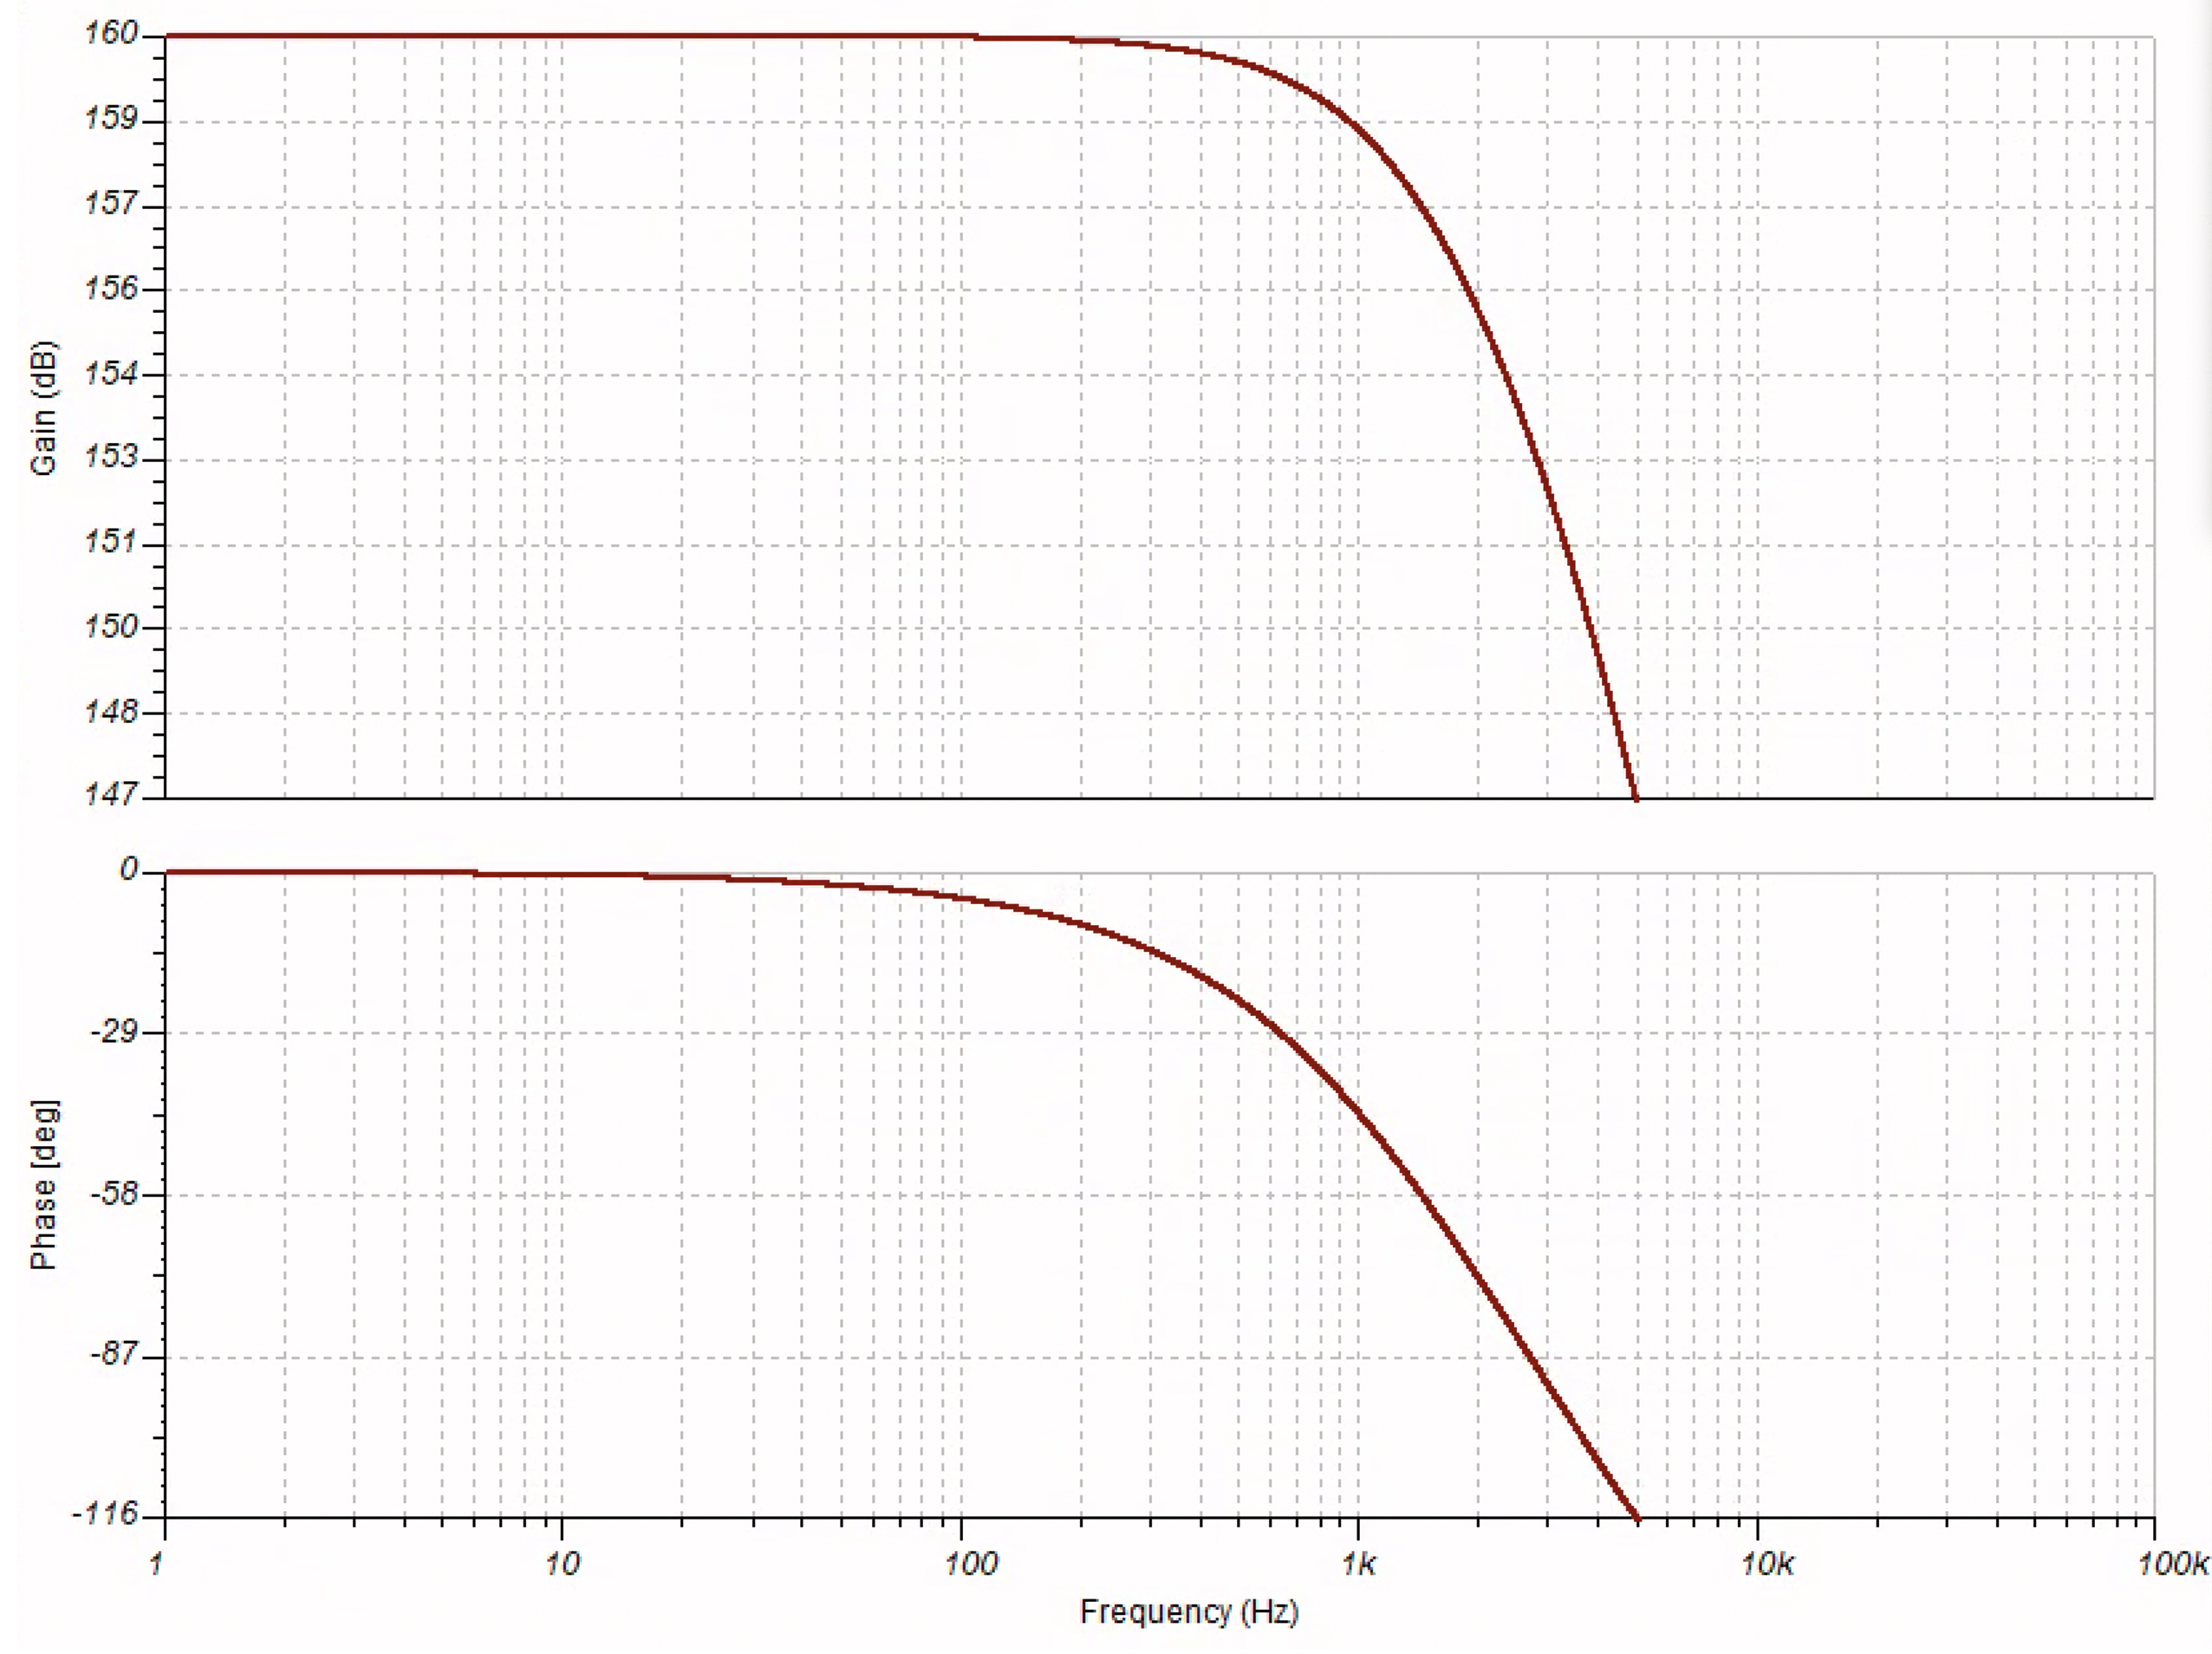
\includegraphics[width=\widthnarrow]{figures/eval/bode.png}
\caption{Amplifier frequency and phase response.}
\label{fig:bodeplot}
\end{figure}

\begin{figure}[t]
\centering
\includegraphics[width=\widthnarrow]{figures/eval/totalnoise.png}
\caption{Total noise of the amplifier vs frequency.}
\label{fig:totalnoise}
\end{figure}

\begin{figure}[t]
\centering
\includegraphics[width=\widthnarrow]{figures/eval/snr.png}
\caption{SNR for an output value of approximately 80~mV (corresponding to a 1~nA photocurrent at 1000~kHz).}
\label{fig:snr}
\end{figure}

\begin{figure}[t]
\centering
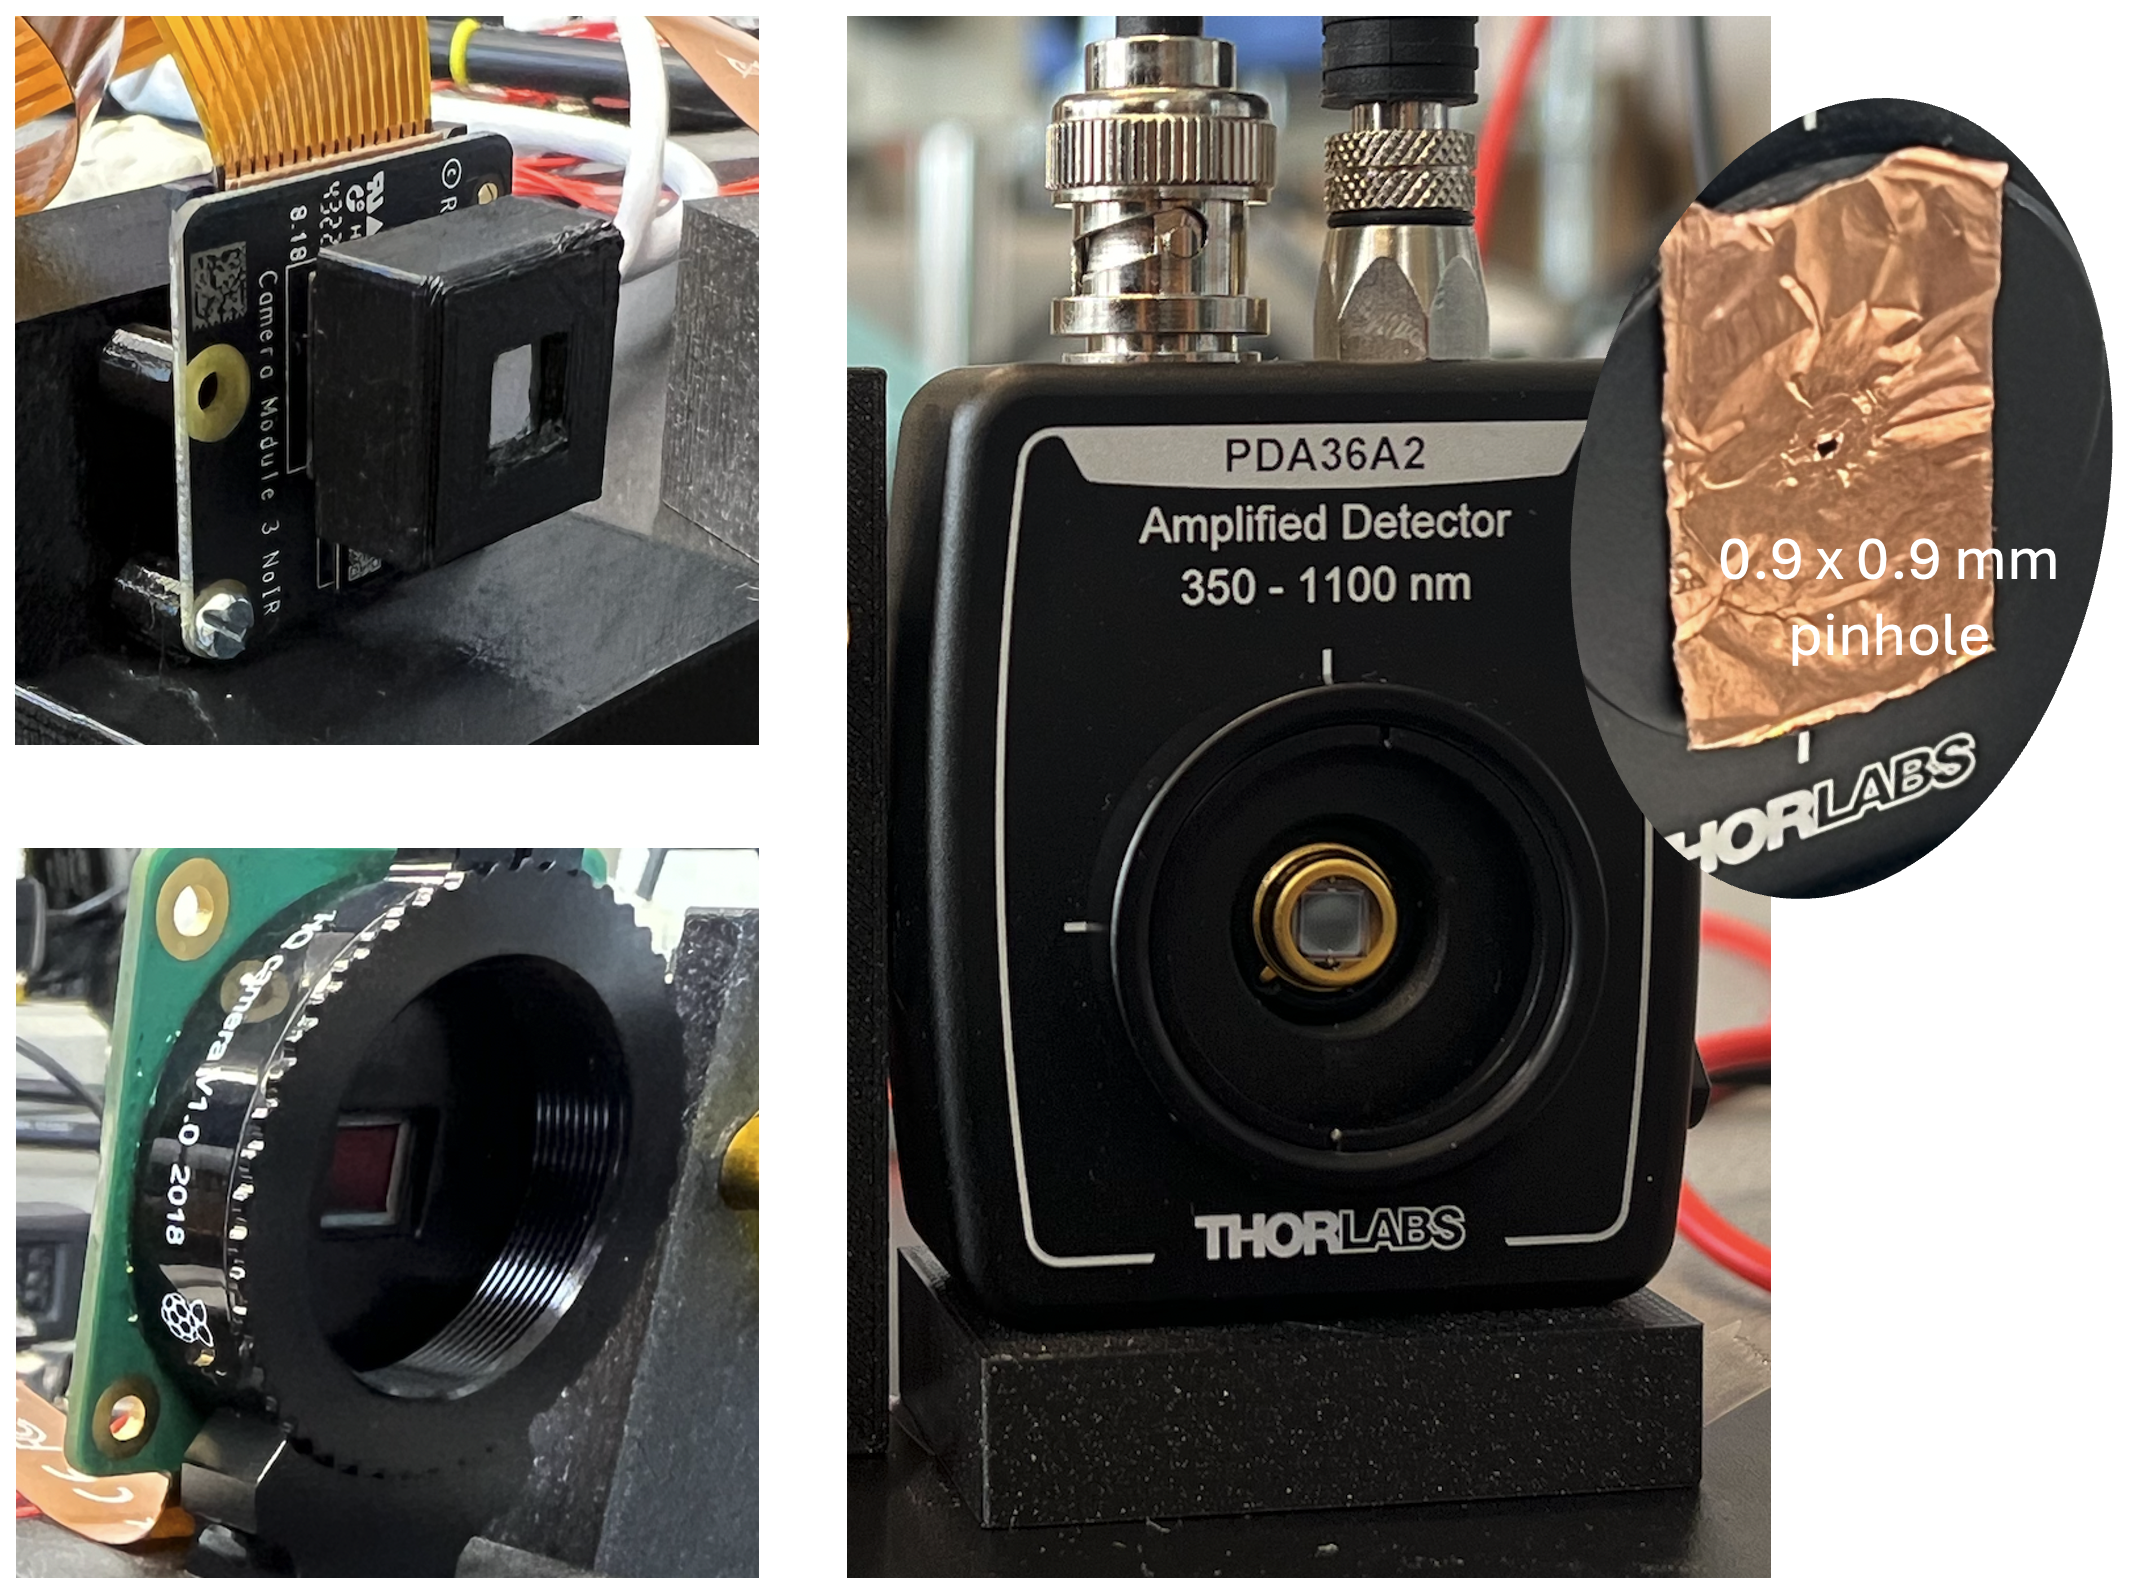
\includegraphics[width=\widthnarrow]{figures/eval/detectors.png}
\caption{Setup of the photodiode array used for detection.}
\label{fig:detectors}
\end{figure}

\begin{figure*}[t]
\centering
\includegraphics[width=\textwidth]{figures/eval/speckles}
\caption{Visualization of speckle patterns under different 1~mW IR laser configurations using the square laser array from Figure~\ref{fig:lasers}. Top left: 1 laser. Bottom right: 10 lasers.}
\label{fig:speckles}
\end{figure*}

\begin{figure*}[t]
\centering
\includegraphics[width=\textwidth]{figures/eval/lasers}
\caption{The different laser setups used from left to right: Red laser for initial emulation experiments, Realsense 415 dot projector with iris, reverse engineered Realsense dot projector and driver circuit, discrete circular and square IR laser arrays.}
\label{fig:lasers}
\end{figure*}
